\subsection{Piezoelectric patches analysis}
\label{subsec:piezoelectric_patches_analysis}

In this section, we introduce the necessary theory to address the use of piezoelectric patches in the system under investigation.

We start by recalling the general constitutive equations for piezoelectric materials before focusing on the specific case of piezoelectric patches bonded to a beam element.

\begin{figure}[H]
    \centering
    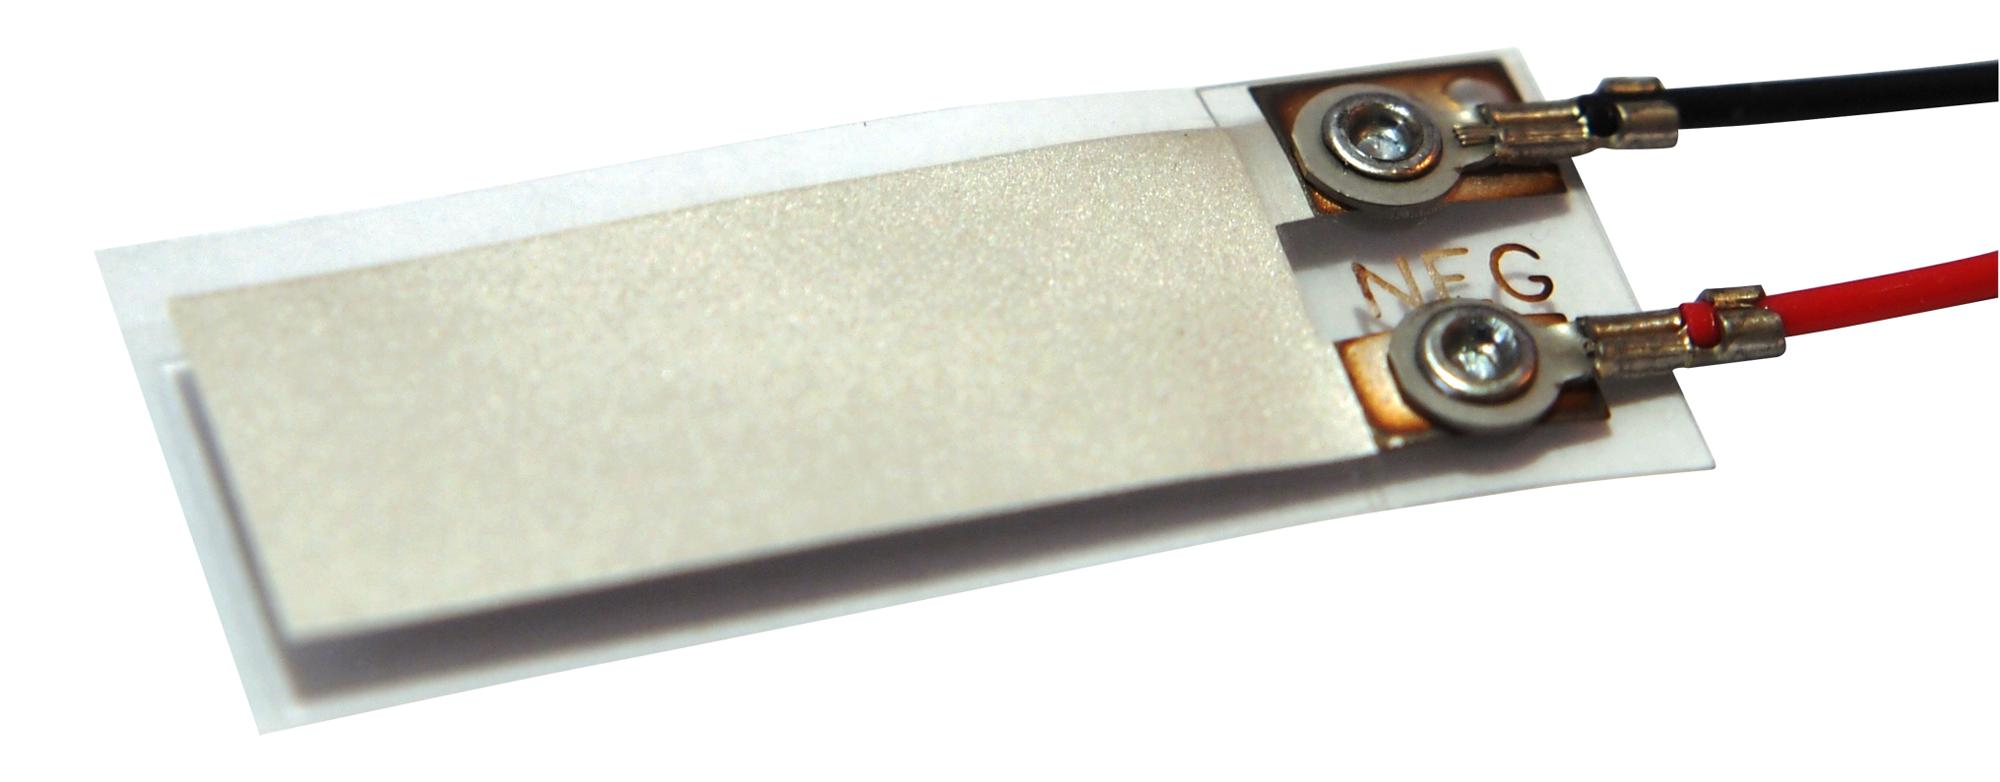
\includegraphics[width=0.5\textwidth]{img/piezo.jpg}
    \caption{Example of piezoelectric patch.}
    \label{fig:piezo}
\end{figure}


\subsubsection{Piezoelectric constitutive equations}
\label{subsubsec:piezoelectric_constitutive_equations}

Piezoelectric materials have the ability to convert mechanical energy into electrical energy and vice versa.
Considering to work within a reasonable range of deformations, the constitutive equations for piezoelectric materials can be linearized and written in matrix form as follows:

\begin{equation}
    \begin{bmatrix}
        \bm{D} \\
        \bm{S}
    \end{bmatrix} =
    \begin{bmatrix}
        \bm{\varepsilon}^T & \bm{d}   \\
        \bm{d}_t           & \bm{s}^E
    \end{bmatrix}
    \begin{bmatrix}
        \bm{E} \\
        \bm{T}
    \end{bmatrix}
\end{equation}

Where $\bm{S} [\Delta m / m]$ and $\bm{D} [C / m^2]$ are the mechanical strain and charge displacement vectors, $\bm{T} [N / m^2]$ and $\bm{E} [N / C]$ are the mechanical stress and electric field vectors, $\bm{s} [1 / Pa]$ is the compliance matrix, $\bm{d} [C / N]$ is the piezoelectric strain coefficient matrix, and $\bm{\varepsilon} [F / m]$ is the dielectric permittivity matrix.
Notice also that the superscript $()^T$ and $()^E$ indicate that the quantities are measured under constant stress and electric field, respectively, while the subscript $t$ indicates the transposition of the matrix.

Taking common assumptions as orthotropy of the material and neglecting any orthogonal piezoelectric effect, the constitutive equations can be greatly simplified forcing many of the coefficients to zero.

For the specific case of piezoelectric patches bonded to a beam element (as will be better shown in Section \ref{subsec:experimental_setup}), we can further simplify the constitutive equations by considering that the electric field is only acting in one direction, and study the stress and strain produced along one of the other normal directions.
In particular, referring to conventional piezoelectric theory, we are interested in the so-called $31$-mode, where the electric field is applied along the $3$-direction and the strain is measured in the $1$-direction (see Figure \ref{fig:piezo_31_operating_mode}).

\begin{figure}[H]
    \centering
    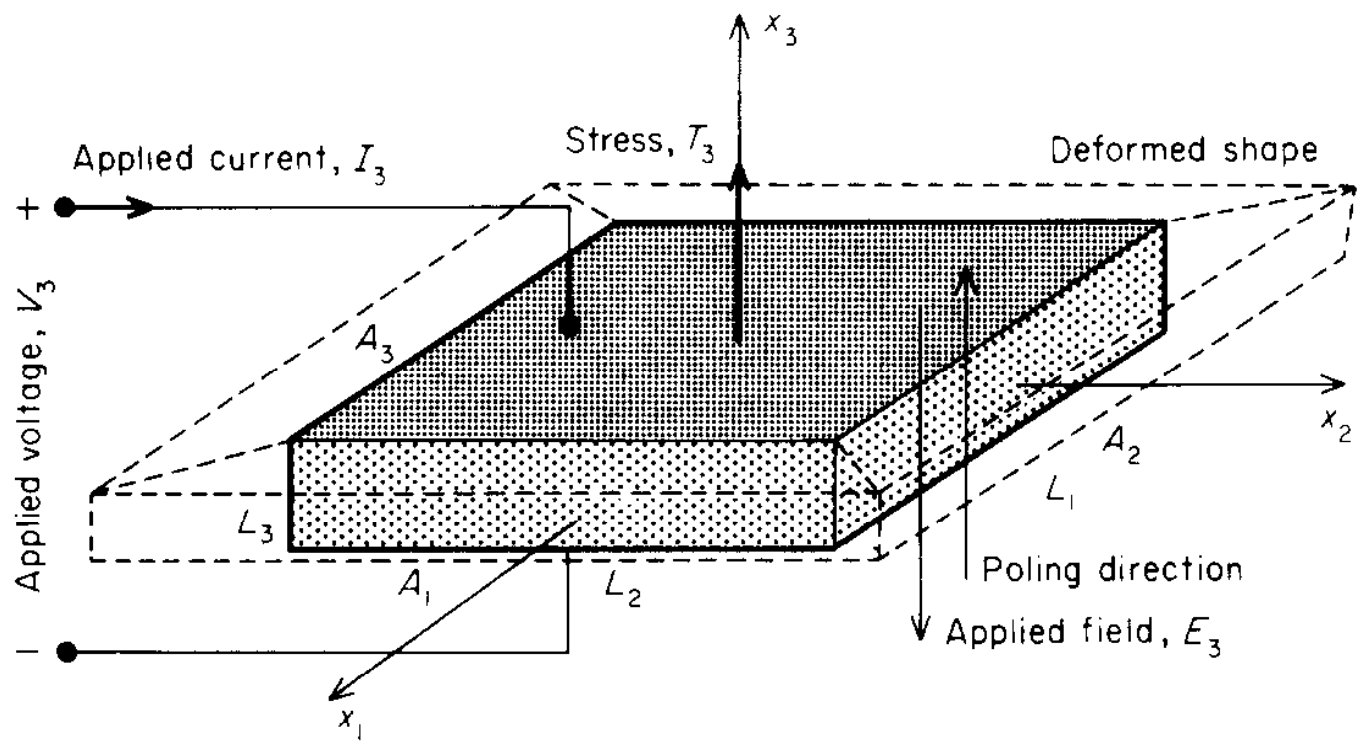
\includegraphics[width=0.7\textwidth]{img/piezo_31_operating_mode.png}
    \caption{Piezoelectric patch operating in $31$-mode.}
    \label{fig:piezo_31_operating_mode}
\end{figure}

Then, under the hypothesis that all the other quantities are zero, the constitutive equations can be written as:

\begin{equation}
    \begin{bmatrix}
        D_3 \\
        S_1
    \end{bmatrix} =
    \begin{bmatrix}
        \varepsilon_{33}^T & d_{31}   \\
        d_{13}             & s_{13}^E
    \end{bmatrix}
    \begin{bmatrix}
        E_3 \\
        T_1
    \end{bmatrix} =
    \begin{bmatrix}
        \varepsilon_{33}^T & d_{31}          \\
        d_{31}             & \frac{1}{Y_1^E}
    \end{bmatrix}
    \begin{bmatrix}
        E_3 \\
        T_1
    \end{bmatrix}
    \label{eq:piezoelectric_constitutive_equations}
\end{equation}

Notice that $\varepsilon_{33}^T$ is the dielectric permittivity in the $3$-direction when the stress in direction $1$ is zero ($T_1 = 0$), and $Y_1^E$ is the Young's modulus in the $1$-direction when the electric field in direction $3$ is zero ($E_3 = 0$).

Equation \ref{eq:piezoelectric_constitutive_equations} can also be rewritten in terms of applied voltage and current by performing the following change of variables and moving to Laplace domain:

\begin{equation}
    \begin{aligned}
        V & = \int_{0}^{L} E \cdot dx & \rightarrow &  & V(s) & = L \cdot E(s)  \\
        I & = \int_A D \cdot dA       & \rightarrow &  & I(s) & = sA \cdot D(s)
    \end{aligned}
\end{equation}

Substituting the expressions for $V$ and $I$ in the constitutive equations, we can obtain the following relationship:

\begin{equation}
    \begin{bmatrix}
        I_3 \\
        S_1
    \end{bmatrix} =
    \begin{bmatrix}
        sC_{3p}^T       & sA_3 d_{31}     \\
        d_{31} L_3^{-1} & \frac{1}{Y_1^E}
    \end{bmatrix}
    \begin{bmatrix}
        V_3 \\
        T_1
    \end{bmatrix}
    \label{eq:piezoelectric_constitutive_equations_volt_current}
\end{equation}

Where $C_p^T = A \varepsilon_{33}^T / L$ is the piezoelectric capacitance per unit length, and $L_3$ is the length of the piezoelectric patch in the $3$-direction.

An important final remark has to be made about the piezoelectric coupling coefficient $k_{31}$, which is defined as:

\begin{equation}
    k_{31} = \frac{d_{31} \sqrt{Y_1^E}}{\varepsilon_{33}^T} = \frac{d_{31}}{\sqrt{\varepsilon_{33}^T Y_1^E}}
\end{equation}

This coefficient is a measure of the efficiency of the piezoelectric material in converting mechanical energy into electrical energy and vice versa.
It's intuitive to understand that $0 < k_{31} < 1$, and the closer it is to $1$, the more efficient the material is in converting energy.


\subsubsection{Shunted piezoelectric patches}
\label{subsubsec:shunted_piezoelectric_patches}

The properties of a piezoelectric patch can be greatly influenced by the presence of a shunt circuit connected to it.
The successive analysis takes as reference the electrical scheme of Figure \ref{fig:shunted_piezoelectric_patch}.

\begin{figure}[H]
    \centering
    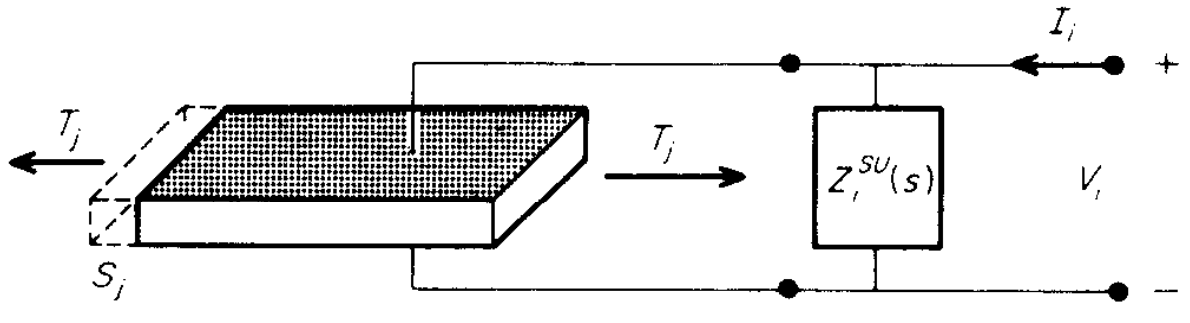
\includegraphics[width=0.7\textwidth]{img/piezo_shunted.png}
    \caption{Electrical scheme of a shunted piezoelectric patch.}
    \label{fig:shunted_piezoelectric_patch}
\end{figure}

In order to account for the presence of the shunt circuit, we need to adjust accordingly the electrical impedance of the system, given now as the parallel connection of the piezoelectric patch impedance $Z_p$ and the shunt impedance $Z_{su}$:

\begin{equation}
    Z^{EL} = \left( Z_p^{-1} + Z_{su}^{-1} \right)^{-1}
\end{equation}

% Or equivalently in terms of admittance:

% \begin{equation}
%     Y^{EL} = Z^{EL^{-1}} = Y_p + Y_{su} = sC_p^T + \frac{1}{Z_{su}}
% \end{equation}

Substituting the expression for $Y^{EL}$ in the constitutive equations (Equation \ref{eq:piezoelectric_constitutive_equations_volt_current}), we obtain the following relationship:

\begin{equation}
    \begin{bmatrix}
        I_3 \\
        S_1
    \end{bmatrix} =
    \begin{bmatrix}
        \frac{1}{Z^{EL}} & sA_3 d_{31}     \\
        d_{31} L_3^{-1}  & \frac{1}{Y_1^E}
    \end{bmatrix}
    \begin{bmatrix}
        V_3 \\
        T_1
    \end{bmatrix}
\end{equation}

Solving for the voltage across the piezoelectric patch, and then for the mechanical strain $S$, we can highlight the influence of the shunt circuit on the mechanical properties of the piezoelectric patch.

\begin{equation}
    \begin{aligned}
        V_3 & = Z^{EL} I_3 - Z^{EL} sA_3 d_{31} T_1                                                                                                                             \\
        S_1 & = d_{31} L_3^{-1} V_3 + \frac{1}{Y_1^E} T_1 = \left( d_{31} L_3^{-1} Z^{EL} \right) I_3 + \left( \frac{1}{Y_1^E} - d_{31} L_3^{-1} Z^{EL} sA_3 d_{31} \right) T_1
    \end{aligned}
\end{equation}

Recalling the traditional definition of stress and strain relationship $S = Y^E T$, we can recognize:

\begin{equation}
    \frac{1}{Y^{SU}} = \frac{1}{Y_1^E} - d_{31} L_3^{-1} Z^{EL} sA_3 d_{31}
\end{equation}

Where $Y^{SU}$ is the mechanical admittance of the piezoelectric patch.
It's clear that the presence of the shunt have a direct influence on the mechanical properties of the piezoelectric patch, and thus on the beam element to which it might be bonded.

In the optic of this work, it's of particular interest to obtain a clear equation of the type $Y^{SU} = f(Y_p, Z_{su})$ that can be used to study the influence of the shunt impedance on the mechanical properties of the piezoelectric patch.
In particular, rearranging the terms of the last equation, we can obtain the following expression:

\begin{equation}
    Y^{SU} = Y_1^D \left( 1 - \frac{k_{31}^2}{1 + s C_p^S Z^{SU}} \right)
    \label{eq:mechanical_admittance_shunted_piezoelectric_patch}
\end{equation}

